

%%%%%%%%%%%%%%%%%%%%%%%%%%%%%%%%%%%%%%%%%%%%%%%%%%%%%%%%%%%%%%%%%%%%%%%%%%%%%%%

%      POINTING

%%%%%%%%%%%%%%%%%%%%%%%%%%%%%%%%%%%%%%%%%%%%%%%%%%%%%%%%%%%%%%%%%%%%%%%%%%%%%%%

\subsection{Pointing}
\label{se:pointing}
% + RTA pointing estimate method
% + pointing model
% + pointing error (scan-to-scan scattering)

\subsubsection{Pointing monitoring}

\begin{figure}[p]
\begin{center}
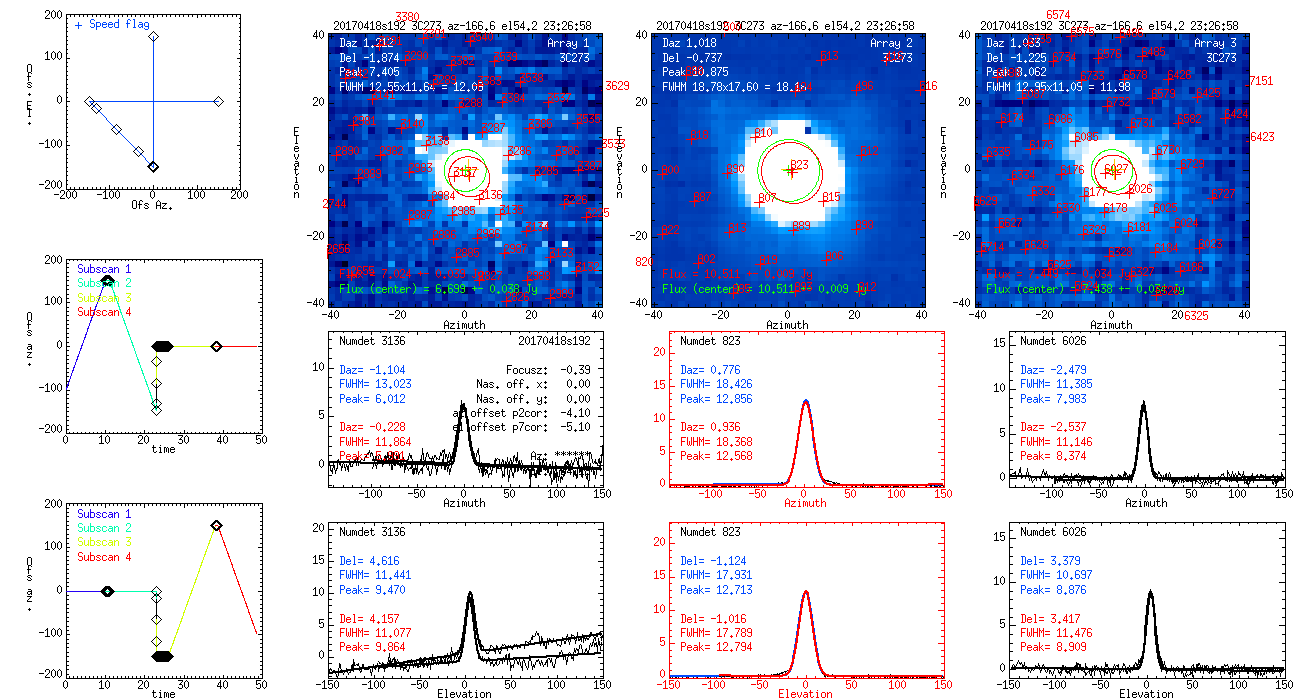
\includegraphics[clip, angle=0, scale = 0.30]{Figures/plot_20170418s192.png}
\caption{Summary plots of the reduction of pointing scan. There is one combined
  map per array to check the overall quality of the scan, and a set of azimuth
  and elevation profiles for one reference detector per array. The 2-mm reference
  detector, highlighed in red, is the the pointing reference detector of
  NIKA2. The location of the peak in azimuth and elevation, as observed by the
  reference detector gives the pointing offset of the current scan.}
\label{fig:ptg}
\end{center}
%\end{figure}
%\begin{figure}[htp]
\begin{center}
\includegraphics[clip, angle=0, scale = 0.70]{Figures/pointing_stats_N2R9.eps}
\caption{Pointing offsets during Run9 observations, before and after the
  derivation of Nasmyth offsets with a pointing session on Feb.~26th, 2017.}
\label{fig:pointing_stats_n2r9}
\end{center}
\end{figure}

Based on general operating experience at the 30-m telescope, we use the so-called
{\em pointing} or {\em cross} scans to monitor the pointing during observations. The
telescope executes a back and forth scan in azimuth and a back and forth scan in
elevation, centered on the observed source. Looking at the timeline profiles of
the reference detector, we fit gaussian profiles and derive the current pointing
offsets of the system in azimuth and elevation. These offsets can then be passed
to PAKO to recenter the next scan (Fig.~\ref{fig:ptg}).

\subsubsection{Pointing session}
Such scans and their analyses are also used to improve the pointing
model of NIKA2. A pointing session consists in observing about 30
sources on a wide range of elevations while monitoring the pointing
offsets that are measured for each observation. These offsets are then
passed to the IRAM staff who finds the pointing model parameters that
minimize and symetrize the scattering of these offsets
(cf.~Fig.~\ref{fig:ptg_scattering}). Bases on these results Nasmyth
offsets are then modified.


Fig.~\ref{fig:pointing_stats_n2r9} shows
the pointing corrections that had to be applied during Run9, before and after
the modification of the Nasmyth offsets. 


While the absolute values of the
corrections is somewhat arbitrary and set around zero for convenience, the
dispersion of the offsets is the true figure of merit of the pointing
corrections. The distribution of corrections after the corrections (in yellow to
red) is clearly more symmetric and narrower than before. During N2R9 run, the pointing accuracy was
1.62 arcsec rms in azimuth and 1.37 arcsec rms in elevation.




\subsection{Focus}


\subsubsection{Axial focus estimation}
\label{sec:focus-meas}

The best axial focus in the central region of the arrays is estimated
using the so-called 'focus$\_$OTF' PAKO script, which realises a
series of five $1' \times 5'$ OTF scans at various values of
the focus in $0.4~\rm{mm}$-steps around an \emph{a priori} value $z_0$,
namely $z \in \{-0.8, -0.4, 0, 0.4, 0.8\} + z_0$. Elliptical Gaussian
fits on the reconstructed maps provide estimates of the flux and FWHM
along minor- and major-axis for each focus. Then, parabolic fits are
used to determine the best focus. We consider three estimates: i)
$\hat z_{\rm{peak}}$ the focus that maximizes the estimated flux,
which is the amplitude of the 2D Gaussian, 
ii) $\hat z_{\rm{fwhm}}$ the focus that
minimizes the geometrical FWHM, defined as the quadratic mean of
$\rm{FWHM}_{\rm{major}}$ and $\rm{FWHM}_{\rm{minor}}$,  and iii)
$\hat z_{\rm{ellipt}}$ the focus that minimizes the beam ellipticity,
defined as $\rm{FWHM}_{\rm{major}}/\rm{FWHM}_{\rm{minor}}$.
Fig.~\ref{fig:focus-example} shows an example of
axial focus measurement using a 'focus$\_$OTF' observation of Neptune
during N2R10.

\begin{figure}
\begin{center}
  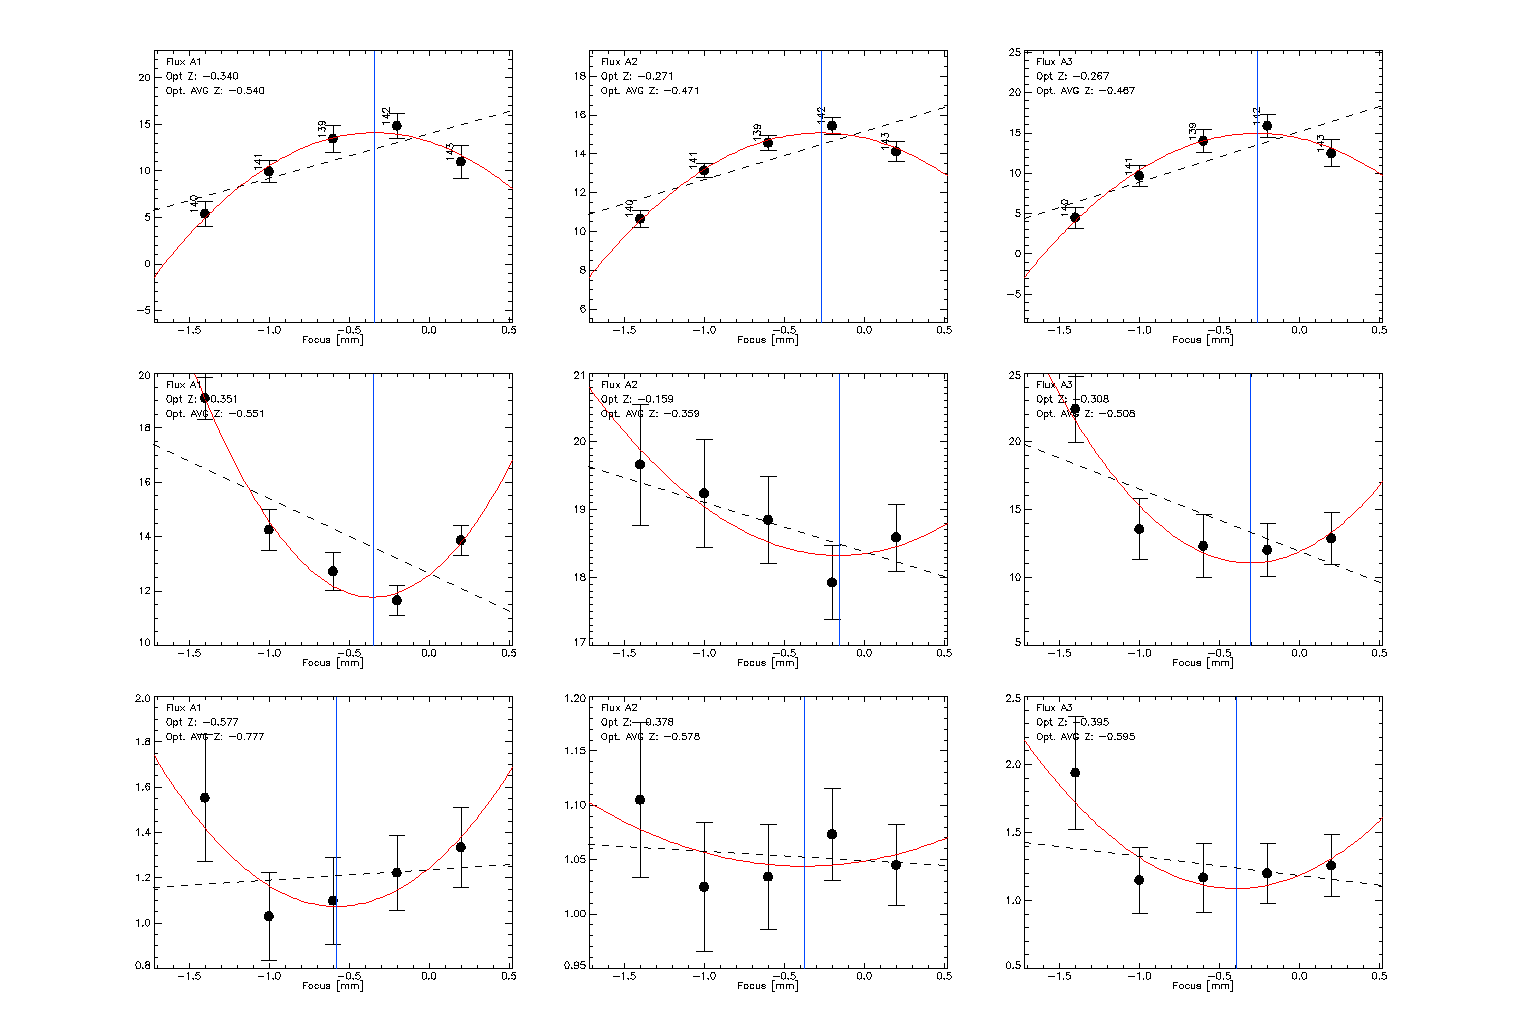
\includegraphics[clip, angle=0, scale=0.25]{Figures/plot_20170419s143.png}
\caption{Example of axial focus measurment using a 'focus$\_$OTF' observation of Neptune
during N2R10 [PLACEHOLDER]}
\label{fig:focus-example}
\end{center}
\end{figure}


\subsubsection{Focus consistency between arrays}

{\bf refaire les plots de difference de focus entre matrices }


\subsubsection{Lateral foci estimation}
\label{sec:focus_X_Y}

{\bf add a description of the method}

{\bf expand a little the discussion below}

Very delicate measurements

The plan is to devote a few hours of technical observation time in
good weather condition to perform an accurate measure of NIKA2 lateral
focus. The X-, Y-focus will then be set at these robust estimated vallues and
checked only a few times a year (at the seasonal change for example).  


Figures \ref{fig:X_focus} and \ref{fig:Y_focus} show examples of the
lateral focus measurements performed during \emph{N2R9}. 

\begin{figure*}[h!]
\centering
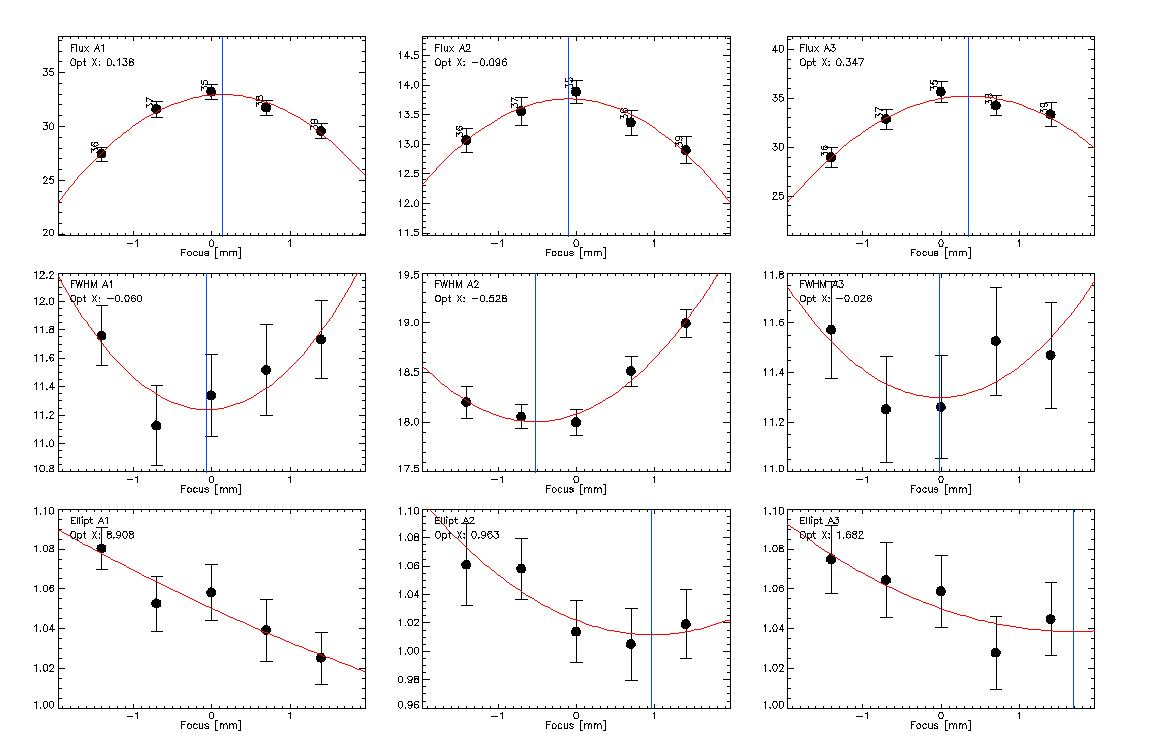
\includegraphics[height=8cm]{Figures/plot_20170223s39.png}
\hspace{0.5cm}
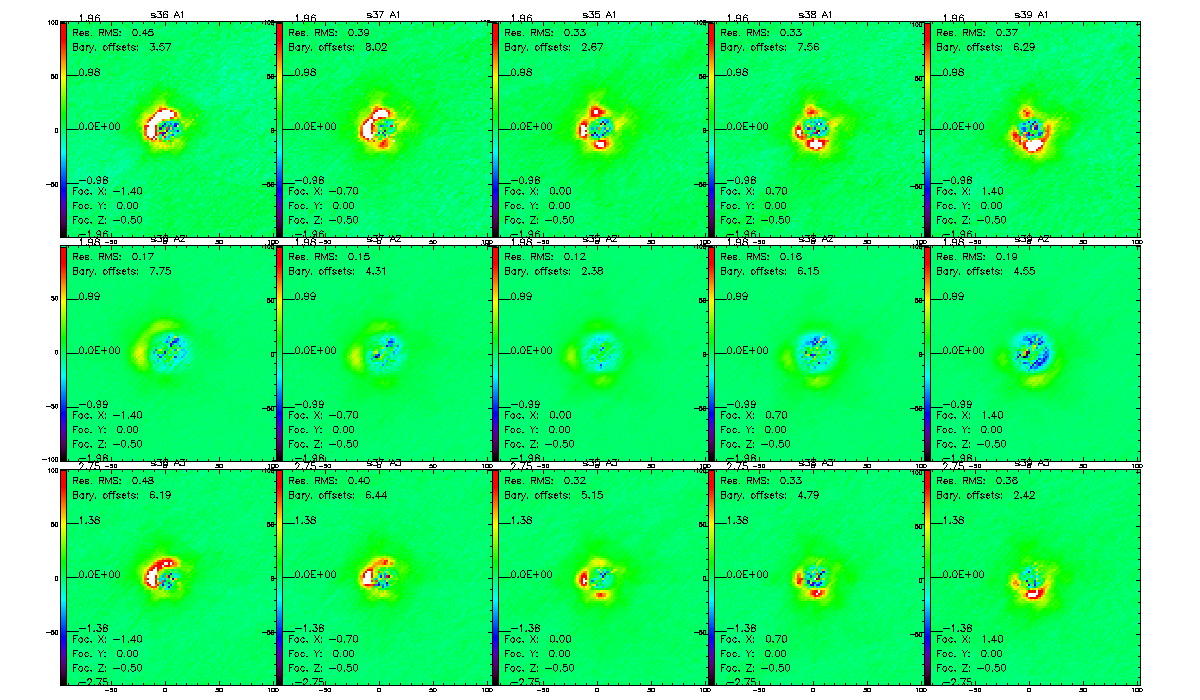
\includegraphics[height=8cm]{Figures/residuals_focus_otf_20170223s39.png}
\caption{{\footnotesize \textbf{Left:} X-focus measurement using a
    parabolic fit of the flux, beam fwhm and ellipticity on a sequence
    of five OTF scans on Uranus (20170223s39-43) \textbf{Right:} Beam residuals after subtracting a model of the main beam for each OTF-scan of the X-focus session.}}
\label{fig:X_focus}
\end{figure*}

\begin{figure*}[h!]
\centering
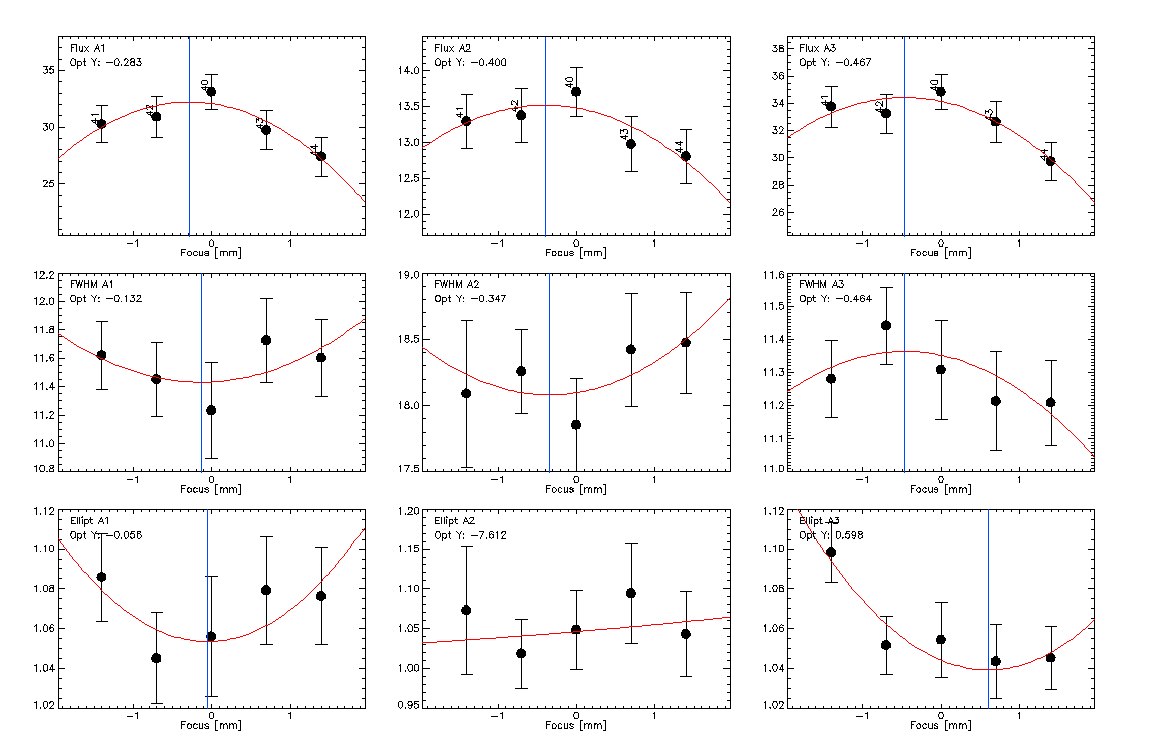
\includegraphics[height=8cm]{Figures/plot_20170223s44.png}
\hspace{0.5cm}
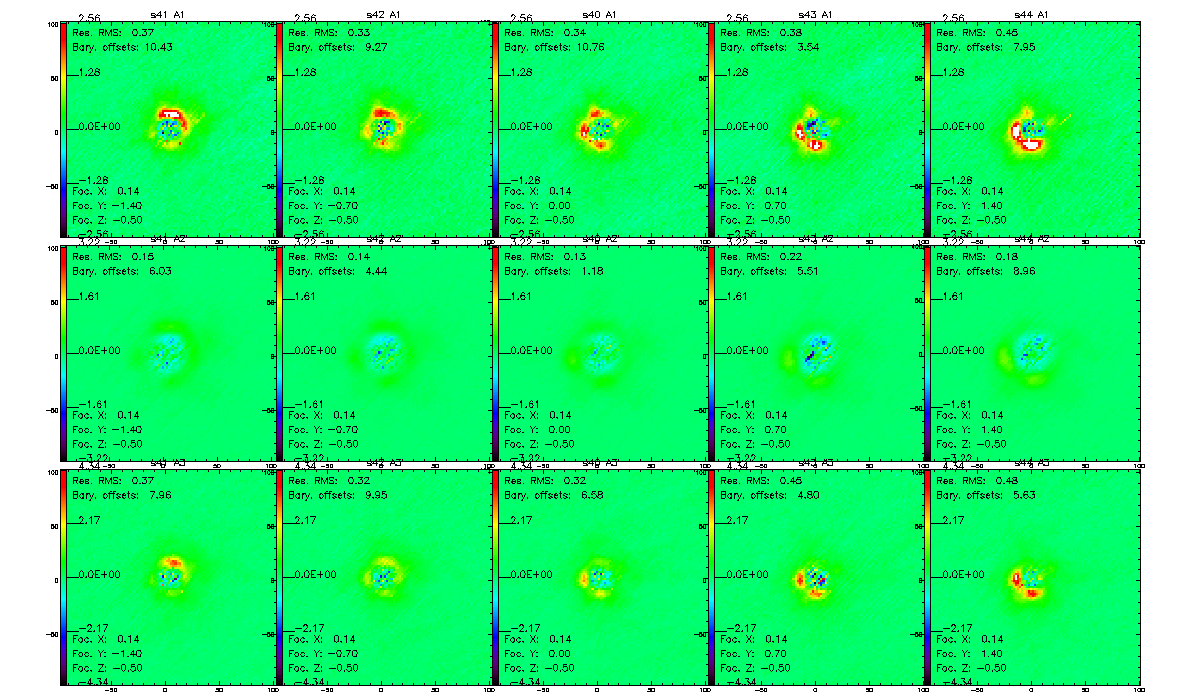
\includegraphics[height=8cm]{Figures/residuals_focus_otf_20170223s44.png}
\caption{{\footnotesize \textbf{Left:} Y-focus measurement using a
    parabolic fit of the flux, beam fwhm and ellipticity on a sequence
    of OTF scans on Uranus (20170223s44-48). \textbf{Right:} Beam residuals after subtracting a model of the main beam for each OTF-scan of the Y-focus session.}}
\label{fig:Y_focus}
\end{figure*}



\subsection{Skydip}




\subsection{Beam maps}

A {\it beammap} is a map a bright and compact source, most of the time
a planet, with an elevation step small enough to meet Nyquist sampling at the 1-mm
beam scale, namely 4.8~arcsec. We observe this planet with a raster scan in
(az,el) coordinates, either with fixed elevation subscans or fixed azimuth
subscans. The former has the advantage of low air mass variation across a
subscan, the latter offers an orthogonal scan direction to the former: the
combination of both gives a more accurate determination of the far side
lobes. 


\subsection{On-The-Flight scan loop}




